\chapter{Реализация программного комплекса}\label{ch:ProgramComplex}

\section{Общая структура программного комплекса}\label{sec:ProgramComplex/GeneralStructure}

В рамках диссертационной работы был реализован конечно-элементный программный комплекс NonLocFEM \cite{NonLocFEM}. Основная задача комплекса --- эффективное решение термомеханических задач в нелокальных постановках на современных вычислительных системах с использованием технологий параллельных вычислений OpenMP \cite{OpenMP} и MPI \cite{MPI}. Все описанные далее методы и алгоритмы реализованы в рамках данного комплекса, а именно: аппроксимация области нелокального влияния; параллельные алгоритмы ассемблирования конечно-элементных матриц; алгоритмы балансировки данных между процессами и потоками исполнения; интегрирование с использованием нестандартных базисов конечных элементов; решатели СЛАУ с использованием специально разработанных предобуславливателей; а также многие другие алгоритмы и методы, на которых не будем заострять слишком много внимания.

Глобальная структура программного комплекса включает в себя математическое ядро и обработчик конфигурационных файлов. Математическое ядро, в свою очередь, также состоит из нескольких взаимосвязанных библиотек, где в качестве основных можно выделить следующие: metamath, parallel, mesh и solvers. В них находятся необходимые примитивы и алгоритмы для конечно-элементных расчётов. Обработчик конфигурационных файлов работает со структурами, представленными в формате JSON \cite{JSONShema} и на их основе формирует запросы для математического ядра, которое проводит необходимые расчёты и возвращает результаты в форматах, которые можно прочитать популярными программами для визуализации данных, например Paraview \cite{Paraview}. Помимо собственных разработок в зависимости комплекса входят две сторонние библиотеки: библиотека линейной алгебры Eigen~\cite{EigenLib} и библиотека для работы со структурами в формате JSON N.~Lohmann~\cite{NlohmannJson}. Схема взаимосвязи модулей программы представлена на Рис.~\ref{pic:NonLocFEMSchema}, где зависимый модуль указывает стрелкой на модуль от которого он зависит.

\begin{figure}[ht]
    \centerfloat{
        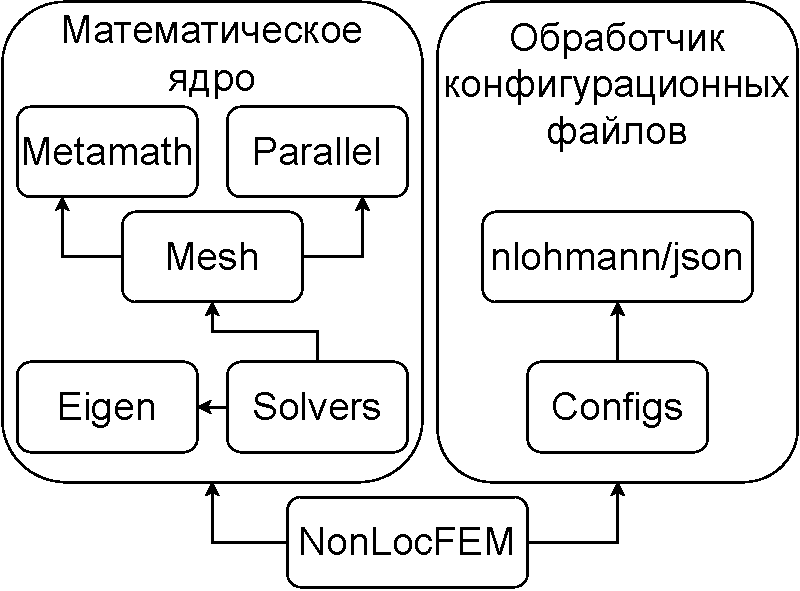
\includegraphics[width=0.7\textwidth]{pics/NonLocFEMSchema.pdf}
    }
    \caption{Структура программы NonLocFEM}\label{pic:NonLocFEMSchema}
\end{figure}

Программный комплекс NonLocFEM реализован на языке программирования C++ \cite{CppReference}. Выбор в пользу этого языка был обоснован его популярностью, богатой стандартной библиотекой, а главное производительностью итоговых программ. Помимо этого, язык предоставляет широкий спектр возможностей в реализации своих идей, особенно если говорить про актуальный на сегодняшний день стандарт языка C++23, возможности которого повсеместно использованы в программном комплексе. Язык C++ мультипарадигменный, поэтому в нём существует возможность совмещать объектно-ориентированные и функциональные подходы к программированию. Объектно-ориентированный подход выражен в виде возможности создания достаточно сложных иерархий классов, в которых могут быть использованы виртуальные методы. Это в свою очередь подразумевает позднее связывание кода программы, то есть во время работы программы могут быть использованы объекты с разной логикой обработки тех или иных данных, имея при этом общий интерфейс. Функциональная парадигма в контексте языка программирования C++ выражена в виде метапрограммирования шаблонов \cite{Alexandresku, Vandevoorde}, где часть вычислений можно вынести на этап компиляции программы, на основе результатов которых генерируется конечный исполняющий файл. Комбинирование двух парадигм открывает возможность совместить такие, порой несовместимые, аспекты программы, как гибкость исходного кода с его производительностью. А учитывая специфику вычислительных программ, в разработке программного комплекса NonLocFEM был сделан достаточно большой уклон в сторону функционых подходов метапрограммирования.

Особенно много приёмов метапрограммирования было использовано в библиотеке metamath, за счёт чего она и получила такое название. В этой библиотеке реализованы различные математические примитивы и функции, а также представлена адаптированная версия библиотеки символьного дифференцирования на этапе компиляции symdiff, основную концепцию которой можно найти в монографии Краснова~М.М.~\cite{KrasnovMeta}. Библиотека symdiff содержит в себе базовые примитивы: константа, переменная; базовые математические операции, такие как  сложение, вычитание, умножение, деление; ряд математических функций, включающих в себя экспоненту, логарифм, тригонометрические функции и многие другие. Благодаря этим примитивам можно строить выражения любой сложности, каждое из которых образует уникальный тип данных. Все эти типы данных объединяет общий интерфейс, предоставляющий возможность вычислить значение этого выражения в точке и посчитать его производную по заданной переменной, при этом вычисление производной порождает новый тип данных, который регистрируется на этапе компиляции программы и соотвествует выражению, являющейся производной исходного выражения. При этом были предприняты меры по оптимизации конечных выражений, сокращающих количество операций, которые необходимы при вычислении значения в точке.

На основе библиотеки symdiff, в рамках библиотеки metamath, была построена библиотека конечных элементов finite\_elements, в которой symdiff использована при описании базисных функций форм элементов и вычислении их производных компилятором. Такой подход значительно упрощает процесс добавления новых элементов, а также сокращает время отладки программы, так как большая часть ошибок, как правило, происходит именно при ручном дифференцировании базисов элементов. Помимо этого такой подход ещё сокращает исходный код программы, так как для добавления нового конечного элемента прикладному программисту необходимо всего лишь описать базис нового элемента в терминах библиотеки symdiff и записать координаты его узлов в локальной системе координат элемента. Для некоторых семейств элементов такой процесс можно автоматизировать, например, для семейства лагранжевых элементов, где базисы элементов построены по определённому алгоритму. Таким образом, можно указать порядок элемента, после чего компилятор сгенерирует необходимый базис в виде набора выражений, которые в дальнейшем могут быть им же и продифференцированы. Помимо дифференцирования базисов, в этой библиотеке также представлен функционал, связанный с процедурой интегрирования. Интегрирование, в отличие от дифференцирования, здесь реализовано численно. Библиотека содержит в себе наборы квадратур разного порядка, при помощи которых выполняется процедура интегрирования. Все элементы и квадратуры, описанные в рамках данной библиотеки, имеют единый интерфейс, поэтому дальнейшие конечно-элементные алгоритмы могут быть записаны в обобщённой форме.

Библиотека mesh предназначена для работы с конечно-элементными сетками. Основным классом данной библиотеки является класс хранилище, объекты которого могут читать файлы с сетками и представлять их в виде, с которым взаимодествуют алгоритмы программы, в том числе и алгоритмы модуля solvers. Схема хранения подразумевает, что элементы образованы путём перечисления номеров узлов, которые им принадлежат, а также ссылкой на объект библиотеки finite\_elements, в котором определены функции формы и квадратурные узлы в локальной системе координат элемента. Также в схеме хранения участвуют координаты узлов сетки и именованные группы элементов, образующих подобласти для определения границ, на которых далее можно задать разные граничные условия. Также было принято решение о том, что в случае использования распределённых вычислений при помощи библиотеки MPI, сетка представлена целиком на каждом отдельном процессе выполнения программы. Такое решение связано с желанием не усложнять схему хранения, ведь для задач в нелокальных постановках, как правило, используются достаточно грубые сетки, содержащие малое количество элементов.

Помимо класса хранилища, в библиотеке mesh также реализованы алгоритмы для работы с конечно-элеметными сетками. Здесь реализованы алгоритмы вычисления квадратурных узлов в глобальной системе координат, вычисления в них якобианов и производных функций форм относительно глобальных переменных. Здесь реализован шаблонный параллельный алгоритм обхода по сетке, на базе которого построены алгоритмы балансировки данных, алгоритм перенумерации узлов Катхилла --- Макки, алгоритм аппроксимации области нелокального влияния и алгоритмы формирования и заполнения портрета конечно-элеметных матриц из модуля solvers. Также в библиотеке mesh реализован функционал сохранения результатов расчётов.

В библиотеке solvers находятся обобщённые алгоритмы ассемблирования матриц и правых частей, и решатели СЛАУ.

Продолжая обзор библиотек программы следует поговорить о библиотеке parallel. Во многом эта библиотека является <<обёрткой>> над библиотеками параллельного программирования OMP и MPI. Она служит двум основным принципам: во-первых, осовременить и обобщить интерфейсы давно устовшихся функций из ранее упомянутых библиотек, которые в современном C++ выглядят весьма громоздко, а во-вторых, собрать все параллельные вызовы в одном месте, что позволяет легко отключать параллелилизм без дополнительных сложностей связанных с компиляцией программы. Кроме того эта библиотека содержит в себе алгоритмы балансировок данных и удобные примитивы для работы с параллельным кодом.

Для связи структур описанных в формате JSON с математическим ядром была разработана библиотека configs. Она содержит в себе примитивы, которые вычисляются на основе JSON и интерпретируются конечной программой в терминах представленных в математическом ядре программы. В случае несоответствия структуры описанной в JSON с ожидаемой библиотека генерирует сообщения об ошибках с указанием места в конфигурационном файле, где возникла эта ошибка.

Для переносимости кода были использованы такие инструменты, как пакетный менеджер Conan \cite{Conan} и система автоматизации сборки \mbox{CMake \cite{CMake}.} Данные инструменты являются кроссплатформенными и распространяются бесплатно, что позволяет легко переносить проект с компьютера на компьютер, а также обеспечивает гибкость в выборе версий сторонних библиотек и настройке компиляции \mbox{проекта.}

\section{Параллельный алгоритм ассемблирования матриц}\label{sec:ProgramComplex/ParallelAlgorithm}

Задачи в нелокальных постановках обладают достаточно большой вычислительной сложностью. Матрицы, получаемые после конечно-элементной аппроксимации, значительно более плотные по сравнению с их классическими аналогами, а также требуют огромных вычислительных ресурсов для их ассемблирования \cite{AMCSM2019}. Поэтому возникает спрос на использование всех возможностей современных компьютеров, а именно параллельные вычисления на машинах с общей и распределённой памятью. Но для того, чтобы полностью задействовать все вычислительные ресурсы, необходимо разработать алгоритм пригодный для распараллеливания.

Для начала упростим аппроксимацию области нелокального влияния $S'(\boldsymbol{x})$, так как рассматриваемый ранее способ квадратурной аппроксимации, описанный формулой (\ref{eq:ApproxNonloc}) и представленный на Рис.~\ref{fig:ApproxSQ}, крайне неудобен для практической реализации. Поэтому возникает идея упростить его и проводить аппроксимацию не относительно квадратурных узлов сетки, а относительно центров элементов. На Рис.~\ref{fig:ApproxSE} крестом обозначен центр элемента относительно которого проводится аппроксимация, область нелокального влияния ограничена окружностью, точками обозначены центры элементов, а серым цветом выделены элементы образующие аппроксимированную область нелокального влияния $S_h^e$. Такой способ аппроксимации будем называть элеметной аппроксимацией. Тогда в алгоритме ассемблирования нелокальной матрицы (\ref{eq:ApproxNonloc}) сможем поменять местами знаки суммирования, после чего сможем преобразовать его к следующему виду
\begin{gather}
	\label{eq:ApproxNonlocByElem}
	\widehat{\textbf{K}}^{NL}_{\mathcal{F}} =
	\sum\limits_{e \in S_h}
	\sum\limits_{n \in I^e}
	\sum\limits_{e' \in S_h^e}
	\sum\limits_{m \in I^{e'}}
	\sum\limits_{q \in Q^e}
	w_q J_q^e
	\sum\limits_{q' \in Q^{e'}}
	w_{q'} \varphi(\boldsymbol{x}_q, \boldsymbol{x}_{q'}) 
	\textbf{K}_{nm}^{e e'}(\boldsymbol{x}_q, \boldsymbol{x}_{q'}) J_{q'}^{e'}.
\end{gather}
Также можем упростить и алгоритм вычисления нелокального температурного линейного расширения (\ref{eq:NonLocalThermalExpansion}) 
\begin{gather}
	\label{eq:NonLocalThermalExpansionByElem}
	\widehat{\textbf{E}}^{NL} = 
	\sum\limits_{e \in S_h}
	\sum\limits_{n \in I^e}
	\sum\limits_{e' \in S_h^e}
	\sum\limits_{q \in Q^e}
	w_q \nabla N_n^e (\boldsymbol{x}_q) J_q^e
	\sum\limits_{q' \in Q^{e'}}
	w_{q'} \varphi (\boldsymbol{x}_q, \boldsymbol{x}_{q'}) \widehat{\mathbf{C}} \cdot \cdot \widehat{\boldsymbol{\alpha}} \Delta T (\boldsymbol{x}_{q'}) J_{q'}^{e'} \boldsymbol{E}_n.
\end{gather}

\begin{figure}[ht]
    \centerfloat{
        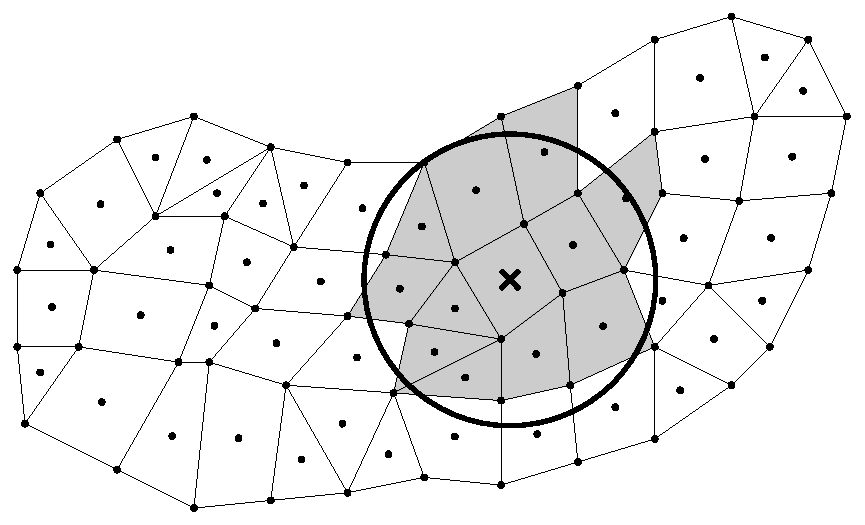
\includegraphics[width=0.7\textwidth]{pics/ApproxSE.pdf}
    }
    \caption{Элементная аппроксимация области нелокального влияния}\label{fig:ApproxSE}
\end{figure}

Такой подход позволяет отделить алгоритм обхода по сетке, ответственного за формирование портрета матрицы, от алгоритма интегрирования, однако, он обладает дефектом, который заключается в том, что не все квадратурные узлы, попадающие в область $S'(\boldsymbol{x}_q)$, центр которой находится в некотором квадратурном узле под номером $q$, попадают под покрытие аппроксимированной области нелокального влияния $S_h^e$. Это может приводить к нарушениям баланса, что в свою очередь приводит к менее точному решению и даже осциляциям. Для решения данной проблемы, радиус поиска соседних элементов нужно брать больше радиуса нелокальности $r$, например, на величину максимального расстояния между центрами двух смежных элементов, где под смежными элементами подразумеваем элементы обладающие хотя бы одним общим узлом. Таким образом, все необходимые квадратурные узлы будут учтены в расчёте.

После разделения алгоритма обхода сетки и алгоритма интегрирования, можем изменить первый таким образом, чтобы сделать его пригодным для параллельных вычислений. Главной проблемой алгоритма (\ref{eq:ApproxNonlocByElem}) остаётся зависимость номера узла сетки от номера текущего элемента из-за чего при использовании параллельных вычислений существует вероятность возникновения гонки данных, что, в зависимости от подхода к распараллеливанию, может приводить к неправильному решению задачи, или частым барьерным синхронизациям, которые в свою очередь снижают эффективность использования параллельных вычислений. Поэтому возникает идея изменить порядок суммирования таким образом, чтобы такой зависимости не было. Для этого определим для каждого узла сетки $n \in S_h$ множество элементов $E^n$, которым он принадлежит и изменим порядок суммирования так, чтобы под первым знаком суммы были номера узлов, а под вторым номера элементов которым он принадлежит
\begin{gather}
	\label{eq:ApproxNonlocParallel}
	\widehat{\textbf{K}}^{NL}_{\mathcal{F}} =
	\sum\limits_{n \in S_h}
	\sum\limits_{e \in E^n}
	\sum\limits_{e' \in S_h^e}
	\sum\limits_{m \in I^{e'}}
	\sum\limits_{q \in Q^e}
	w_q J_q^e
	\sum\limits_{q' \in Q^{e'}}
	w_{q'} \varphi(\boldsymbol{x}_q, \boldsymbol{x}_{q'}) 
	\textbf{K}_{nm}^{e e'}(\boldsymbol{x}_q, \boldsymbol{x}_{q'}) J_{q'}^{e'}.
\end{gather}
Такой алгоритм сборки матрицы является построчным, соответственно каждую строку матрицы можно собирать независимо в своём исполняемом потоке, а также распределить вычисление строк между вычислительными узлами.

Полученный алгоритм (\ref{eq:ApproxNonlocParallel}) пригоден для параллельных вычислений на машинах с общей и распределённой памятью, однако, возникает проблема балансировки данных и объёма вычислений. При решении этих проблем стоит начинать с проблемы балансировки данных, так как из-за неё есть вероятность возникновения ситуации, когда задача не может быть решена, в силу того, что на одном из вычислительных узлов может не хватить оперативной памяти, в то время как при балансировке данных такой проблемы можно было бы избежать.

При балансировке данных будем исходить из гипотезы, что на каждом вычислительном узле $p \in P$ установлено одинаковое количество оперативной памяти и данные нужно распределить равномерно между всеми вычислительными узлами $P$. Для этого необходимо найти общее число элементов матрицы $M$, затем найти среднее $M_m = M / |P|$ и распределить строки матрицы между вычислительными узлами таким образом, чтобы в каждой группе строк количество элементов матрицы было приблизительно равным $M_p \approx M_m$. На практике удобнее всего брать группы последовательных строк. Причём при балансировке нет необходимости формировать полный портрет матрицы, это также можно делать построчно, что гораздо эффективнее и легко реализовать. Также при балансировке необходимо учесть симметрию полученной матрицы, так как из-за достаточно больших объёмов выгодно хранить лишь её половину.

После балансировки данных между вычислительными узлами, можем также провести балансировку объёмов вычислений между вычислительными потоками. Для этого необходимо проделать ту же процедуру, что и при балансировке данных, но осреднять не по количеству элементов матрицы, а по количеству вызовов функции интегрирования. В некоторых ситуациях такая балансировка может быть полезна и между вычислительными узлами, например, когда сборка матрицы занимает гораздо больше времени, чем решение итоговой СЛАУ.

Вместе с параллельным алгоритмом ассемблирования нелокальных матриц (\ref{eq:ApproxNonlocParallel}), можем также выписать параллельный алгоритм ассемблирования локальных матриц (\ref{eq:LocalMatrix})
\begin{gather*}
	\widehat{\textbf{K}}^L_{\mathcal{F}} =
	\sum\limits_{n \in S_h}
	\sum\limits_{e \in E^n}
	\sum\limits_{m \in I^e}
	\sum\limits_{q \in Q^e}
	w_q \textbf{K}^{ee}_{nm} (\boldsymbol{x}_q, \boldsymbol{x}_q) J_q^e,
\end{gather*}
Аналогично можно поступить и с ассемблированием матрицы теплообмена (\ref{eq:HeatTransferMatrix}), а также векторами в правой части (\ref{eq:HeatTransferVector}) --- (\ref{eq:OuterFlux}) уравнения теплопроводности (\ref{eq:ThermalSLAE})
\begin{gather*}
	\textbf{Q} =
	\sum\limits_{n \in S_h}
	\sum\limits_{e \in E^n}
	\sum\limits_{q \in Q^e}
	w_q q_V (\boldsymbol{x}_q) J_q^e \boldsymbol{E}_n,
\end{gather*}
\begin{gather*}
	\textbf{F} =
	\sum\limits_{n \in \Gamma_h}
	\sum\limits_{e \in E^n}
	\sum\limits_{q \in Q^e}
	w_q f (\boldsymbol{x}_q) J_q^e \boldsymbol{E}_n,
\end{gather*}
\begin{gather*}
	\widehat{\textbf{K}}^{\alpha}_T =
	\sum\limits_{n \in \Gamma_h}
	\sum\limits_{e \in E^n}
	\sum\limits_{m \in I^{e}}
	\sum\limits_{q \in Q^e}
	w_q \alpha N_n^e (\boldsymbol{x}_q) N_m^e (\boldsymbol{x}_q) J_q^e \boldsymbol{E}_n \otimes \boldsymbol{E}_m,
\end{gather*}
\begin{gather*}
	\textbf{T}^{\alpha} =
	\sum\limits_{n \in \Gamma_h}
	\sum\limits_{e \in E^n}
	\sum\limits_{q \in Q^e}
	w_q \alpha N_n^e (\boldsymbol{x}_q) T_{\alpha} (\boldsymbol{x}_q) J_q^e \boldsymbol{E}_n.
\end{gather*}
Проделаем те же выкладки и для векторов правой части (\ref{eq:InnerPressure}) --- (\ref{eq:LocalThermalExpansion}) и (\ref{eq:NonLocalThermalExpansionByElem}) уравнения равновесия (\ref{eq:StressSLAE})
\begin{gather*}
	\widehat{\textbf{B}} =
	\sum\limits_{n \in S_h}
	\sum\limits_{e \in E^n}
	\sum\limits_{q \in Q^e}
	w_q \boldsymbol{b} (\boldsymbol{x}_q) J_q^e \boldsymbol{E}_n,
\end{gather*}
\begin{gather*}
	\widehat{\textbf{P}} = 
	\sum\limits_{e \in \Gamma_h}
	\sum\limits_{n \in I^e}
	\sum\limits_{q \in Q^e}
	w_q \boldsymbol{p} (\boldsymbol{x}_q) J_q^e \boldsymbol{E}_n,
\end{gather*}
\begin{gather*}
	\widehat{\textbf{E}}^L = 
	\sum\limits_{n \in S_h}
	\sum\limits_{e \in E^n}
	\sum\limits_{q \in Q^e}
	w_q \nabla N_n^e (\boldsymbol{x}_q) \cdot \widehat{\mathbf{C}} \cdot \cdot \widehat{\boldsymbol{\alpha}} \Delta T (\boldsymbol{x}_q) J_q^e \boldsymbol{E}_n,
\end{gather*}
\begin{gather*}
	\widehat{\textbf{E}}^{NL} = 
	\sum\limits_{n \in S_h}
	\sum\limits_{e \in E^n}
	\sum\limits_{e' \in S_h^e}
	\sum\limits_{q \in Q^e}
	w_q \nabla N_n^e (\boldsymbol{x}_q) J_q^e \cdot
	\sum\limits_{q' \in Q^{e'}}
	w_{q'} \varphi (\boldsymbol{x}_q, \boldsymbol{x}_{q'}) \widehat{\mathbf{C}} \cdot \cdot \widehat{\boldsymbol{\alpha}} \Delta T (\boldsymbol{x}_{q'}) J_{q'}^{e'} \boldsymbol{E}_n,
\end{gather*}
Отметим, что при ассемблировании векторов на каждом вычислительном узле можем также ограничиться только теми строками, которые были получены при балансировке.

\section{Алгоритм аппроксимации области нелокального влияния}\label{sec:ProgramComplex/SearchMeighbours}

При аппроксимации области нелокального влияния необходимо использовать метод поиска ближайших соседей, однако, важно выбрать оптимальный для рассматриваемых задач алгоритм. Наивный алгоритм линейного поиска имеет квадратичную сложность $O (N^2)$, в связи с чем на достаточно подробных сетках время поиска может быть весьма существенным. Поэтому построим алгоритм поиска в основе которого лежит k-d дерево \cite{kdtree}.

Суть метода на основе k-d дерева заключается в разделении пространства занимаемого телом на равномерные ячейки, после разбиения на которые необходимо составить списки узлов соответствующие ячейкам, в которых они оказались. Размер ячеек следует брать равным радиусу поиска, тогда при поиске ближайших соседей поиск можно ограничить до ячейки в которой находится этот узел и смежных ей ячейкам. В качестве алгоритма поиска внутри ячеек можно использовать обычный линейный поиск, тогда сложность такого алгоритма можно оценить как $O(N \log N)$, что на подробных сетках заметно быстрее линейного поиска. Пример разбиения представлен на Рис. \ref{fig:SearchNeighbours}, где крестом указан рассматриваемый узел, тёмно-серым цветом выделена ячейка, которой принадлежит этот узел, а светло-серым смежные ей ячейки, область нелокального влияния ограничена окружностью.

\begin{figure}[ht]
    \centerfloat{
        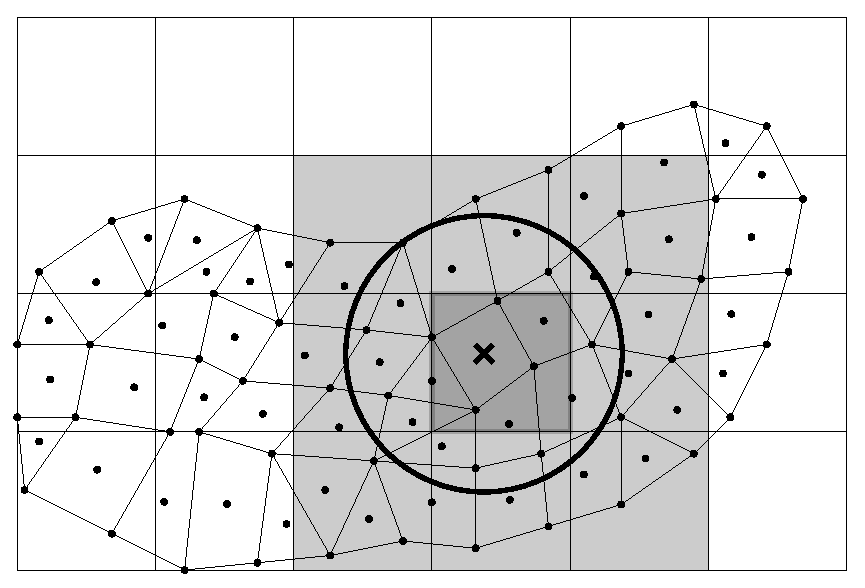
\includegraphics[width=0.7\textwidth]{pics/SearchNeighbours.pdf}
    }
    \caption{K-d дерево для поиска ближайших соседей}\label{fig:SearchNeighbours}
\end{figure}

\section{Оптимизация базисных функций конечных элементов}\label{sec:ProgramComplex/BasisOptimization}

Помимо эффективных алгоритмов сборки матрицы жёсткости, также возникает потребность в эффективном решении итоговых СЛАУ. Прямые методы, применённые к разреженным матрицам, как правило требуют значительных затрат оперативной памяти, поэтому возникает спрос на использование итерационных методов решения \cite{Demmel}. Однако итерационные методы могут иметь слишком медленную сходимость, которая в первую очередь обусловлена самой системой. Таким образом возникает идея уменьшить число обусловленности системы и как правило для этого используют разного рода предобуславливатели и адаптируют сетку таким образом, чтобы элементы были ближе к своим исходным формам \cite{MeshOptimization1, MeshOptimization2}. Также для ускорения сходимости можно подобрать начальные данные, чтобы они были как можно точнее к искомому решению. Но в случае, когда для вычислений используют элементы высшего порядка, появляется дополнительная возможность оптимизировать базис элемента под конкретную задачу.

Обычно использование элементов высшего порядка может быть связано с желанием более точно аппроксимировать искомые величины или производные от этих величин, такие как тепловые потоки или деформации \cite{HighOrderElements1, HighOrderElements2}. Также они могут понадобиться для решения специфических задач, где могут встречаться производные высшего порядка. В задачах не обладающих такой спецификой большой популярностью обладают квадратичные серендиповые элементы, так как они позволяют достаточно точно аппроксимировать градиенты искомых функций и при этом, как показано на Рис.~\ref{fig:QuadraticSerendipity}, не имеют внутренних узлов, что заметно упрощает расчёты.

\begin{figure}[ht]
    \centerfloat{
        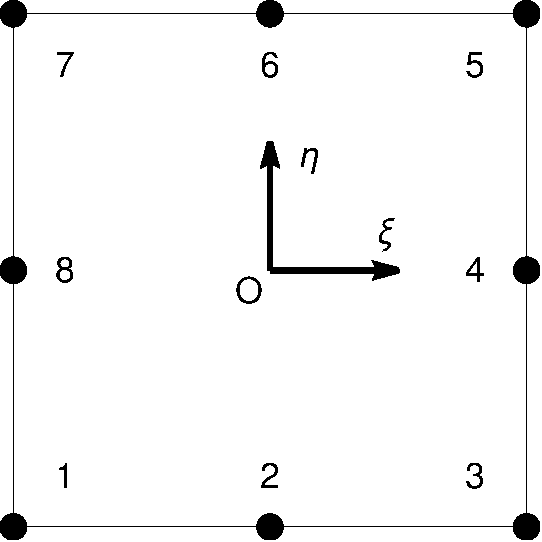
\includegraphics[width=0.5\textwidth]{pics/QuadraticSerendipity.pdf}
    }
    \caption{Квадратичный серендиповый элемент в локальной системе координат $\text{O}\xi\eta$}\label{fig:QuadraticSerendipity}
\end{figure}

Набор базисных функций для квадратичного серендипового элемента, которые предложил O.~Zienkiewicz \cite{Zienkiewicz}, не единственный и к тому же обладает рядом дефектов, которые повышают число обусловленности итоговой системы уравнений. Поэтому рассмотрим семейство базисных функций с дополнительным параметром $s$ \cite{QuadraticSerensipity}
\begin{gather*}
    N_i = \dfrac{1}{16} (1 + \xi_i \xi) (1 + \eta_i \eta) ((9s - 1) (1 - \xi_i \xi - \eta_i \eta) + (9s + 3) \xi_i \xi \eta_i \eta), \\ 
    i = 1, 3, 5, 7; \xi_i, \eta_i = \pm 1, \\
    N_i = \dfrac{1}{16} (1 - \xi^2) (1 + \eta_i \eta) ((5 - 9s) + (9s + 3)\eta_i \eta),
    \quad
    i = 2, 6; \ \eta_i = \pm 1, \\
    N_i = \dfrac{1}{16} (1 - \eta^2) (1 + \xi_i \xi) ((5 - 9s) + (9s + 3)\xi_i \xi),
    \quad
    i = 4, 8; \ \xi_i = \pm 1.
\end{gather*}
Выбор параметра $s$ был основан на следующих предположениях
\begin{gather*}
    \int\limits_{-1}^{1} \int\limits_{-1}^{1} N_i (\xi, \eta) d\xi d\eta = s,
    \quad
    i = 1, 3, 5, 7, \\
    \int\limits_{-1}^{1} \int\limits_{-1}^{1} N_i (\xi, \eta) d\xi d\eta = 1 - s,
    \quad
    i = 2, 4, 6, 8.
\end{gather*}
Таким образом, классический базис можно получить при $s = -1 / 3$.

Теперь можем перейти к задаче минимизации числа обусловленности матриц теплопроводности $\widehat{\textbf{K}}_T$ и жёсткости $\widehat{\textbf{K}}_E$, которые для удобства дальнейшего изложения будем обозначать одной буквой $\widehat{\textbf{K}}$. Для этого введём понятие числа обусловленности, как квадратный корень отношения максимального по модулю собственного числа $\lambda_{\max}$ к минимальному по модулю собственному числу $\lambda_{\min}$ матрицы $\widehat{\textbf{K}}$
\begin{gather}
	\label{eq:CondValue}
	\operatorname{cond} \widehat{\textbf{K}} = \sqrt{\dfrac{|\lambda_{\max}|}{|\lambda_{\min}|}}.
\end{gather}

Воспользуемся гипотезой, что минимальное по модулю собственное число $\lambda_{min}$ слабо зависит от параметров модели и дополнительного параметра базиса. Так как след матрицы равен сумме её собственных значений, а сама матрица симметричная и положительно определённая, то задача минимизации числа обусловленности эквивалентна задаче минимизации следа матрицы
\begin{gather*}
    \min\limits_s \operatorname{tr} \widehat{\mathbf{K}} =
    \min\limits_s \sum\limits_{e \in S_h} \int\limits_{S^e} \sum\limits_{i = 0}^k \sum\limits_{j = 0}^2 c_{j} N^e_{i,j} d S^e,
\end{gather*}
где $k$ --- количество функций форм элемента, $c_{j}$ --- некоторые постоянные коэффициенты, зависящие от свойств материала. Но, как легко заметить, результат задачи оптимизации не зависит от количества элементов и их геометрических свойств (считаем, что сетка состоит из однородных элементов), поэтому можем упростить задачу и рассмотреть лишь один элемент в локальной системе координат. Таким образом, для квадратичного серендипового элемента задача оптимизации сводится к поиску минимума квадратичной параболы
\begin{gather}
	\label{eq:ParamSOptimal}
	\min\limits_s \int\limits_{-1}^{1} \int\limits_{-1}^{1} \sum\limits_{i = 0}^8 \sum\limits_{j = 0}^2 c_{j} N_{i, j}^2(\xi, \eta) d\xi d\eta =
	\min\limits_s C (27 s^2 -12 s + 19) \
	\rightarrow \ s = \dfrac{2}{9},
\end{gather}
где $C$ --- некоторая константа. Исходя из полученной оценки, ожидаемый минимум числа обусловленности, а также наибольшая скорость сходимости итерационных методов решения СЛАУ должна быть в окрестности точки $s = 2/9$.